\documentclass[10pt] {article}
\usepackage{fourier}
\author{Ankit Goyal \\ankit@cs.utexas.edu \\ CS380L}
\title{Lab 3: Program loading and memory mapping}
\date{\today}	
\usepackage{full page}
\usepackage{minted} % to insert code
\renewcommand\listingscaption{Codeblock}



\usepackage{hyperref, url}
\usepackage{listings}
\usepackage{graphicx}
\usepackage{caption}
\usepackage{subcaption}
\usepackage{amsmath}
%\usepackage{amsmath, enumerate, url, ulem, algorithmic, polynom, subfig}

\setlength\parindent{0pt}

\begin{document}
\maketitle
%----------------------------------------------------------------------------------------
%  Specs
%----------------------------------------------------------------------------------------

\section{Setup}
\subsection{Hardware}
\textbf{Host Processor}: 64 bit 4 core Intel(R) Xeon(R) CPU E3-1270 V2 @ 3.50GHz\\
\textbf{Host Memory}: 16GB \\
\textbf{HyperThreading}: Yes \\
\textbf{Logical CPUs after Hyperthreading}: 8 \\
\textbf{CPU frequency scaling}: Disabled in BIOS (turned off Intel SpeedStep and C-states)

\subsection{Software}
\textbf{Host Operating System}: Ubuntu with 3.13.0-34-generic 64 bit kernel.\\

\section{Creating the memory image of a new process}

\texttt{sys\_execve} is responsible for setting up the environment for running the program. Below are the steps taken by \texttt{sys\_execve} which calls  \texttt{do\_execve\_common}:

\begin{enumerate}
\item Check that \texttt{NPROC} limit is not exceeded (i.e., total number of process), if it is then exit. (L: 1443)
\item Allocate memory for data structure in kernel. (L: 1458) 
\item Open the \texttt{exec} file using \texttt{do\_open\_exec} (L: 1469)
\item Now the kernel data structures are initialized and \texttt{exec\_binprm} is called. 
\item \texttt{exec\_binprm} calls \texttt{search\_binary\_handler} which finds the binary format handler, in our case elf. So it finds \texttt{load\_elf\_binary}. (fs/binfmt\_elf.c L:84 \& 571)
\begin{itemize}
\item \texttt{load\_elf\_binary} does consistency checks by making sure that it's an ELF format file by comparing the main number and ELF in \texttt{e\_ident} field in header.
\item \texttt{load\_elf\_binary} reads the header information and looks for \texttt{PT\_INTERP} segment to see if an interpreter was specified. This segment is only present for dynamically linked programs and not for statically linked.
\item Now all the loadable segments are \texttt{mmapped} into memory, by reading the ELF Program headers. \texttt{bss} segment is also mapped.
\item \texttt{create\_elf\_tables} creates a stack at a random offset and sets the auxiliary vectors, arguments and environments according to the standard.
\item Finally the control is transferred to \texttt{e\_entry} point using \texttt{start\_thread} method.(fs/binfmt\_elf.c L:990)
\end{itemize}
\end{enumerate}

\section{Implemented Loaders}
\subsection{All at Once Loader}
In this all the pages were mapped while loading the test program including \texttt{bss}. 
\textbf{On calling malloc}, memory is allocated by kernel and not the loader program. The process executes successfully.

\subsection{On-demand Loader}
In this loader, at startup only the first page is mapped. A \texttt{segfault handler} is registered and when the program tries to access an unmapped page, it segfaults and the \texttt{segfault handler} maps the corresponding address from file. Performance is discussed later\\

\subsection{Hybrid Loader}
In this loader, at startup all text and initialized data is mapped. The \texttt{bss} memory is mapped on demand. \\

\textbf{If a program tries to access an invalid memory address}, the \texttt{segmentation fault} is propagated and is thrown as a user would expect. \\

Hybrid loader also uses the following prediction algorithm, where on every successful prediction a counter is increased and it allows us to map pages in advance.


\begin{listing}[ht!]
\begin{minted}{cpp}

int correctPredictions = 0;

void pagePrediction(unsigned long currentAddress){
	if (last_prediction_was_correct)
		correctPredictions++;
	else 
		correctPredictions--;
		
	if (correctPredictions == 1){
		map next 1 page
	} else if (correctPredictions > 1) {
		map next 2 pages
	}
	predict the next page to be 1 page after the last mapped page
}

\end{minted}
\label{lst:sched}
\caption{Prediction Algorithm}
\end{listing}

\section{Test Programs and Results}
Following section first describes the program and then the results of running each loader on that program. All the results in this section refer to Fig. 1 %Last page gives the actual numbers received after running these programs.

\begin{figure}[ht!]
\centering
\begin{subfigure}{.5\textwidth}
\centering
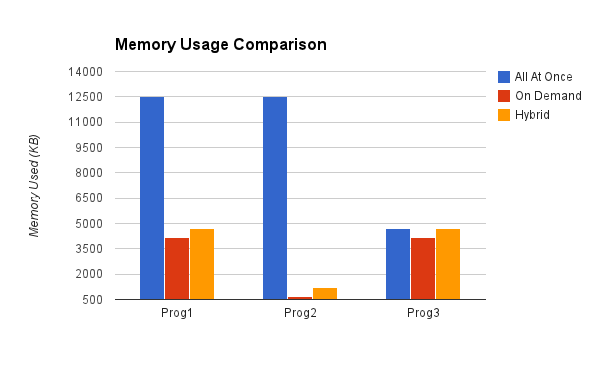
\includegraphics[width=\linewidth]{img1.png}
\caption{}
\label{fig:thvsfair1}
\end{subfigure}%
\begin{subfigure}{.5\textwidth}
\centering
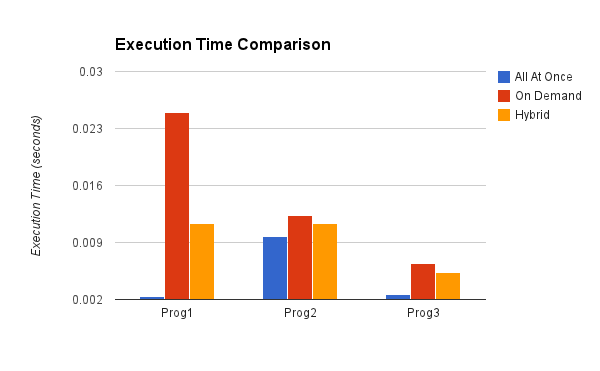
\includegraphics[width=\linewidth]{img2.png}
\caption{}
\label{fig:thvsfair2}
\end{subfigure}
\caption{Memory Usage and Execution Time comparison for three loaders}
\label{fig:thvsfair}
\end{figure}

\subsection{\texttt{prog1}}
\texttt{prog1} contains 3 uninitialized global variables (large bss segment). It accesses only one of the arrays. This shows the effect of loading all the pages in memory rather than getting them on demand or through some heuristic. This program makes printf call to make sure that it runs correctly.
\begin{enumerate}
\item \textbf{All at once} uses a large amount of memory when compared to other two since it maps everything on startup. The execution time of all at once is less because the memory is already mapped and the program doesn't segfault as in other two cases.
\item \textbf{On Demand} uses the least amount of memory since the memory is mapped only when needed. Since the program seagulls more often and it has an overhead associated with it. It can be seen that the execution time of On-demand is greater than the other two due to this overhead.
\item \textbf{Hybrid} maps only the text and data segment while loading. Since the array is accessed sequentially it is able to predict quite well and is using almost the same amount of memory as used by demand paging. Due to the decrease in overhead due to segfaults, it's execution time is better than on-demand loader. 
\end{enumerate}

\begin{listing}[ht!]
\begin{minted}{cpp}
int a[1000000];
int b[1000000];
int c[1000000];

int main() {
	int i;
	for (i=0; i<1000000; i++) {
		a[i] = 12;
	}
	printf("hello!\n");
 }
\end{minted}
\label{lst:sched}
\caption{prog1}
\end{listing}


\subsection{\texttt{prog2}}
\texttt{prog2} contains 3 uninitialized global variables (large bss segment). It accesses only one of the arrays but in a random order and accesses only a part of it. This shows the variation in performance of hybrid pages.

\begin{enumerate}
\item \textbf{All at once}: Again all-at-once uses a large amount of memory when compared to other two since it maps everything on startup. The execution time of all at once is less because the memory is already mapped and the program doesn't segfault as in other two cases.
\item \textbf{On Demand} uses the least amount of memory since the memory is mapped only when needed. Randomness doesn't affect on-demand since it only maps pages when they are needed.
\item \textbf{Hybrid} maps only the text and data segment while loading. Since the array is accessed randomly it not is able to predict as effectively as the \texttt{prog1} given the nature of the algorithm. 
\end{enumerate}


\begin{listing}[ht!]
\begin{minted}{cpp}
int a[1000000];
int b[1000000];
int c[1000000];

int main() {
	int xRan;
	srand(time(0));
	int i;
	for (i=0; i<1000000/2; i++) {
		xRan = rand()%100000;
		a[xRan] = 12;
	}
 }
\end{minted}
\label{lst:sched}
\caption{prog2}
\end{listing}

\subsection{\texttt{prog3}}  
\texttt{prog3} contains a simple array that loops through it. The memory usage of each method should be equivalent in this case.
\begin{enumerate}
\item \textbf{All at once} Since almost all the \texttt{bss} memory is accessed, at the end all three loaders map all the pages. All-at-once uses the same amount of memory and it's execution is again better due to the same reasons. 
\item \textbf{On Demand} On-demand has a high overhead and since we are mapping the whole memory it has the worse execution time.
\item \textbf{Hybrid} has a higher overhead than all at once but less than on-demand. This is reflected in the execution time and again it uses the same amount of memory.
\end{enumerate}

\begin{listing}[ht!]
\begin{minted}{cpp}
static int a[1000000];
int main() {
	for (i=0; i<1000000; i++) {
    		a[i] = 12;
  	}
}
\end{minted}
\label{lst:sched}
\caption{prog3}
\end{listing}


\subsection{\texttt{prog4}}  
\texttt{prog4} is the code given on course page. This code throws a segmentation fault when run. All three loaders throw a \texttt{segmentation fault}

When demand or hybrid pager gets \texttt{segfault}, they check if the given faulting address belongs to a address in the loaded file. If not, they \texttt{raise} the signal \texttt{SIGSEGV} again. Since it's a double fault, the program aborts throwing a segmentation fault to the user. 

\begin{listing}[ht!]
\begin{minted}{cpp}
int
main() {
   int *zero = NULL;
   return *zero;
}
\end{minted}
\label{lst:sched}
\caption{prog4}
\end{listing}

\section {Actual Numbers in the Graph}

\subsection{Execution Time (seconds)}
\begin{tabular}{llll}

 & Prog1 & Prog2 & Prog3 \\
All At Once & 0.002344 & 0.009721 & 0.002592 \\
On Demand & 0.024904 & 0.012285 & 0.006405 \\
Hybrid & 0.011381 & 0.011351 & 0.005276 \\
\end{tabular}

\subsection{Memory Usage (KB)}

\begin{tabular}{llll}

 & Prog1 & Prog2 & Prog3 \\
All At Once & 12506 & 12509 & 4693 \\
On Demand & 4176 & 652 & 4172 \\
Hybrid & 4704 & 1192 & 4696 \\
\end{tabular}

\vfill

\noindent \textbf{Time Spent on the lab \ensuremath{\approx} 30 hours} 

\section{References}
\begin{enumerate}
  \item http://eli.thegreenplace.net/2012/08/13/how-statically-linked-programs-run-on-linux/
  \item http://www.skyfree.org/linux/references/ELF\_Format.pdf
  \item http://linux.die.net/man/5/elf
  \item http://articles.manugarg.com/aboutelfauxiliaryvectors.html
  \item  http://pubs.opengroup.org/onlinepubs/009695399/functions/sigaction.html
  \item http://stackoverflow.com/questions/8116648/why-is-the-elf-entry-point-0x8048000-not-changeable
  \item http://lxr.free-electrons.com/source/fs/exec.c\#L1425
\end{enumerate}

\end{document}